\section{Theorie}
\label{sec:Theorie}

% In knapper Form sind die physikalischen Grundlagen des Versuches, des Messverfahrens, sowie sämtliche für die Auswertung erforderlichen Gleichungen darzustellen. (Keine Herleitung)

% (eventuell die Aufgaben)

% Der Versuchsaufbau: Beschreibung des Versuchs und der Funktionsweise (mit Skizze/Bild/Foto)

Der Compton Effekt beschreibt die Streuung eines Photons an einem Elektron.
Beim Stoß mit dem Elektron gibt das Photon Energie ab und dessen Wellenlänge wird größer.
Die Größe dieser Veränderung hängt vom Streuwinkel $\Theta$ ab, wobei $\Theta=\SI{0}{\degree}$ bedeutet, dass die Bahn des Photons nicht verändert wurde. (siehe \autoref{fig:compton})
Wenn $\lambda_1$ die Wellenlänge vor dem Stoß und $\lambda_2$ die Wellenlänge nach dem Stoß beschreibt, lässt sich die Differenz über
\begin{equation}
    \Delta \lambda = \lambda_2 - \lambda_1 = \frac{h}{m_e c}(1-\cos \Theta)
    \label{eq:differenz}
\end{equation}
berechnen.
Der Vorfaktor ist proportional zu den Naturkonstanten der Lichtgeschwindigkeit $c$, dem Planckschen Wirkungsquantum $h$ und der Elektronenmasse $m_e$.
Dieser konstante Vorfaktor 
\begin{equation}
    \lambda_c = \frac{h}{m_e c}
    \label{eq:compton-wellenlänge}
\end{equation}
heißt Compton Wellenlänge.

\begin{figure}
    \centering
    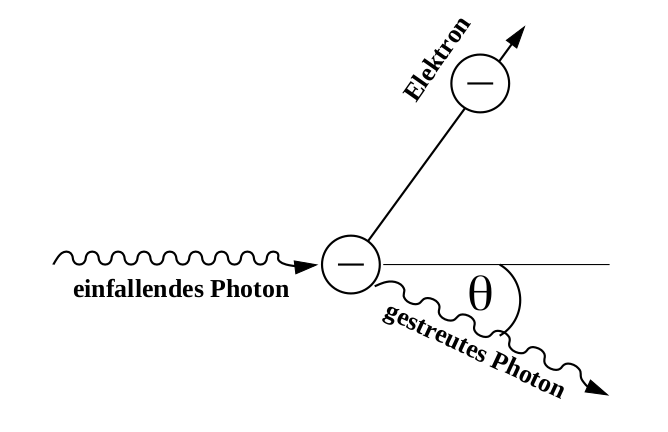
\includegraphics[width=0.4\textwidth]{images/bild_1.png}
    \caption{Schematische Darstellung des Compton Effekts.\cite{V603}}
    \label{fig:compton}
\end{figure}

Um den Effekt beobachten zu können wird hier Röntgenstrahlung an Plexiglas und einem LiF-Kristall gestreut. 
Die ausfallende Strahlung wird über ein Geiger-Müller-Zählrohr und über die Transmission durch eine Aluminiumplatte mit der einfallenden Strahlung verglichen.
Diese Röntgenstrahlung wird in einer Röntgenröhre erzeugt, in der Elektronen von einer Glühkathode auf eine Anode beschleunigt werden. 
Der Zusammenstoß auf der Anode erzeugt $\gamma$-Strahlung.

Das Spektrum dieser Strahlung hängt vom Material der Anode ab.
Dieses ist zwar kontinuierlich, allerdings sind zwei Maxima in der Intensität deutlich zu erkennen, 
da diese Photonenenergien gerade der Energiedifferenz der Energieniveaus eines Anodenatoms entspricht.
Dies ist so zu erklären, dass diese Energien benötigt werden damit das stoßende Elektron ein Elektron aus dem Atom herrausschlägt.
Damit die so entstandene Lücke geschlossen werden kann, muss die Energie gerade der Energiedifferenz zwischen zwei Energieniveaus der Schalen im Schalenmodell des Atoms entsprechen.

Um die Wellenlänge $\lambda$ mit einer Photonenenergie in Verbindung zu bringen wird 
\begin{equation}
    E = \frac{h c}{\lambda}
    \label{eq:photonenenergie}
\end{equation} 
verwendet.

Um das charakteristische Spektrum der hier verwendeten Kupferanode zu bestimmen, wird die Röntgenstrahlung an einem LiF-Kristall gebeugt.
Hierbei entsteht beim Glanzwinkel $\alpha$ eine konstruktive Interferenz, welche von der Wellenlänge der Röntgenstrahlung abhängt. 
Die zugehörige Wellenlänge zum Winkel $\alpha$ kann über 
\begin{equation}
    \lambda = \frac{2d}{n}\sin\alpha
    \label{eq:glanzwinkel}
\end{equation}
bestimmt werden. 
Hier ist $d$ die Gitterkonstante des Kristalls und $n$ die Beugungsordnung.

Der Geiger-Müller-Zähler kann die Strahlung nicht kontinuierlich messen, sondern hat eine Totzeit $\tau$.
Daher muss dies über
\begin{equation}
    I = \frac{N}{1 - \tau N}
    \label{eq:totzeit}
\end{equation}
korrigiert werden. Hier ist $N$ die Anzahl der Anschläge des Geiger-Müller-Zählers und $I$ die Intensität der Strahlung.\cite{V603}